\documentclass{article}%
\usepackage[T1]{fontenc}%
\usepackage[utf8]{inputenc}%
\usepackage{lmodern}%
\usepackage{textcomp}%
\usepackage{lastpage}%
\usepackage{authblk}%
\usepackage{graphicx}%
%
\title{Chronic Morphine Treatment Attenuates Cell Growth of Human BT474 Breast Cancer Cells by Rearrangement of the ErbB Signalling Network}%
\author{Jason Campbell}%
\affil{Instituto de Biologa Molecular y Celular de Plantas, Universidad Politcnica de Valencia{-}C.S.I.C, Ciudad Politcnica de la Innovacin, Valencia, Spain}%
\date{01{-}01{-}2013}%
%
\begin{document}%
\normalsize%
\maketitle%
\section{Abstract}%
\label{sec:Abstract}%
SAN DIEGO {-} Researchers at San Diego State University have found signs in humans that point to specific sources of protein from which those cells develop.\newline%
"Most cancer cells probably do not produce cancer{-}causing proteins," said Sam Savran, MD, Ph.D., postdoctoral researcher in the department of bioengineering. "The fact that these genes are found in many cancer cells is surprising. As a matter of fact, when we screened a wide range of cancer cell types, we saw only one that evolved in that way."\newline%
The study published in the March issue of Oncotarget explains that tumor cells whose T{-}cells derived from "chaotic regions" of normal cells usually are cancerous. Meanwhile, cells with the T{-}cells of one particular type are high in protein. But these abnormal T{-}cells in cancer and other varieties show signs of the functional markers HLA{-}C and TCR and of missing protein in protein{-}dependent cells.\newline%
"As with other types of DNA damage, cancer patients go through a phase of repair," said Ann L. Croman, MD, PhD, a postdoctoral fellow in the Department of Cellular, Molecular and Molecular Physiology. "This work is one more indication that standard cellular therapies may not work well for certain cancers."\newline%
To identify the key sources of T{-}cell signaling, the researchers developed new algorithms, which translate signals into a fluorescent tag that is worn by the cells. They then analyzed the data using an artificial high energy printer (noninvasive or surgically infused dye) for antigen{-}antitrypsin levels in active T{-}cells from two groups of human breast cancer patients.\newline%
"These high T{-}cell signaling pathways are unlike those found in other cancers," Savran said. "They are central to the development of many types of cancer."\newline%
Savran said that this discovery could help determine which therapies work best in those patients and which could be administered as a monotherapy and in combination with checkpoint inhibitors.\newline%
The study was funded by the National Cancer Institute, the American Cancer Society, Cancer Prevention Program of the National Institutes of Health and Discovery Fund of the California Institute for Regenerative Medicine.

%
\subsection{Image Analysis}%
\label{subsec:ImageAnalysis}%


\begin{figure}[h!]%
\centering%
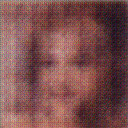
\includegraphics[width=150px]{500_fake_images/samples_5_474.png}%
\caption{A Black And White Photo Of A Black And White Cat}%
\end{figure}

%
\end{document}